% Please add the following required packages to your document preamble:
% \usepackage[normalem]{ulem}
% \useunder{\uline}{\ul}{}

\iffalse
\begin{table*}[]
  \centering
  \begin{tabular}{|c|c|c|c|c|c|c|c|c|c|c|}
      \hline
      \textit{Metric}                                                            & \textit{\begin{tabular}[c]{@{}c@{}}Connected\\ components\end{tabular}} & \textit{\begin{tabular}[c]{@{}c@{}}Global\\ cc\end{tabular}} & \textit{\begin{tabular}[c]{@{}c@{}}Approx.\\ global cc\end{tabular}} & \textit{\begin{tabular}[c]{@{}c@{}}Average\\ cc\end{tabular}} & \textit{\begin{tabular}[c]{@{}c@{}}Local\\ cc's\end{tabular}} & \textit{Degree} & \textit{\begin{tabular}[c]{@{}c@{}}Close-\\ ness\end{tabular}} & \textit{\begin{tabular}[c]{@{}c@{}}Between-\\ ness\end{tabular}} & \textit{\begin{tabular}[c]{@{}c@{}}Page-\\ Rank\end{tabular}} & \textit{\begin{tabular}[c]{@{}c@{}}Eigen-\\ vector\end{tabular}} \\ \hline
      \textbf{\begin{tabular}[c]{@{}c@{}}Execution\\ time\end{tabular}}          & 57s                                                                     & 56s                                                          & 56s                                                                      & 1m 02s                                                        & 1m 2s                                                         & 1m 03s          & \begin{tabular}[c]{@{}c@{}}20h 39m\\ 37s\end{tabular}          & \begin{tabular}[c]{@{}c@{}}4d 10h\\ 31m 12s\end{tabular}         & 1m 28s                                                        & 1m 16s                                                           \\ \hline
      \textbf{\begin{tabular}[c]{@{}c@{}}RAM\\ consumption\\ (MBs)\end{tabular}} & 246.11                                                                  & 246.89                                                       & 247.43                                                                   & 302.21                                                        & 313.58                                                        & 297.90          & 331.02                                                         & 371.27                                                           & 508.70                                                        & 324.11                                                           \\ \hline
      \end{tabular}
  \caption{Execution time and RAM consumption of the metric computations on the CAPRI cluster.}
  \label{tab:capri}
\end{table*}
\fi

\begin{table*}[]
  \centering
  \begin{tabular}{|c|c|c|c|c|c|}
      \hline
      \textbf{\#}           & \textit{\textbf{1}}                                        & \textit{\textbf{2}}                                         & \textit{\textbf{3}}                                           & \textit{\textbf{4}}                                         & \textit{\textbf{5}}                                    \\ \hline
      \textit{Degree}       & Johann Sebastian Bach                                      & Traditional                                                 & Mc Gw                                                         & MC MN                                                       & Jean Sibelius                                          \\ \hline
      \textit{Closeness}    & R3HAB                                                      & Snoop Dogg                                                  & Diplo                                                         & David Guetta                                                & Tiësto                                                 \\ \hline
      \textit{Betweenness}  & Snoop Dogg                                                 & Traditional                                                 & R3HAB                                                         & Diplo                                                       & Johann Sebastian Bach                                  \\ \hline
      \textit{PageRank}     & Johann Sebastian Bach                                      & Traditional                                                 & Jean Sibelius                                                 & Mc Gw                                                       & MC MN                                                  \\ \hline
      \textit{Eigenvector}  & Farruko                                                    & French Montana                                              & Gucci Mane                                                    & Ty Dolla \$ign                                              & Lil Wayne                                              \\ \hline
      \textit{Average rank} & \begin{tabular}[c]{@{}c@{}}Snoop Dogg\\ (5.8)\end{tabular} & \begin{tabular}[c]{@{}c@{}}Gucci Mane\\ (11.6)\end{tabular} & \begin{tabular}[c]{@{}c@{}}David Guetta\\ (18.8)\end{tabular} & \begin{tabular}[c]{@{}c@{}}Steve Aoki\\ (19.0)\end{tabular} & \begin{tabular}[c]{@{}c@{}}Diplo\\ (20.8)\end{tabular} \\ \hline
      \end{tabular}
  \caption{Top 5 artists in the whole dataset, according to our centrality measures. The "average rank" row also reports the value for each artist.}
  \label{tab:ranking}
  \end{table*}

\begin{table*}[]
    \centering
    \begin{tabular}{|c|c|c|c|c|c|c|c|}
    \hline
    \textbf{Reference graph}                                                       & \textit{Average cc} & \textit{Global cc} & \textit{\begin{tabular}[c]{@{}c@{}}Approximate\\ global cc\end{tabular}} & \textit{\begin{tabular}[c]{@{}c@{}}Maximum\\ eigenvector\end{tabular}} & \textit{\begin{tabular}[c]{@{}c@{}}Average\\ eigenvector\end{tabular}} & \textit{\begin{tabular}[c]{@{}c@{}}Maximum\\ closeness\end{tabular}} & \textit{\begin{tabular}[c]{@{}c@{}}Average\\ closeness\end{tabular}} \\ \hline
    \textbf{House subgraph}                                                        & \xmark              & \cmark             & \cmark                                                                   & \cmark                                                                 & \cmark                                                                 & \cmark                                                               & \cmark                                                               \\ \hline
    \textbf{Pop subgraph}                                                          & \xmark              & \xmark             & \xmark                                                                   & \cmark                                                                 & \cmark                                                                 &                                                                      &                                                                      \\ \hline
    \textbf{Rap subgraph}                                                          & \xmark              & \xmark             & \xmark                                                                   & \cmark                                                                 & \cmark                                                                 & \cmark                                                               & \xmark                                                               \\ \hline
    \textbf{Whole dataset}                                                         & \xmark              & \xmark             & \xmark                                                                   & \cmark                                                                 & \cmark                                                                 &                                                                      &                                                                      \\ \hline
    \textbf{\begin{tabular}[c]{@{}c@{}}Top 10\%\\ popularity subgraph\end{tabular}} & \xmark              & \xmark             & \xmark                                                                   & \cmark                                                                 & \cmark                                                                 & \xmark                                                               & \xmark                                                               \\ \hline
    \textbf{Trap subgraph}                                                         & \xmark              & \xmark             & \xmark                                                                   & \cmark                                                                 & \cmark                                                                 & \cmark                                                               & \xmark                                                               \\ \hline
    \end{tabular}
    \caption{Results of the Shapiro-Wilk normality tests for all considered graphs. The "reference graph" is the graph to which the random graphs used in the analysis refer to. "cc" stands for "clustering coefficient".}
    \label{tab:normality}
\end{table*}

\begin{table*}[]
  \centering
  \begin{tabular}{|c|c|c|c|c|c|c|c|}
  \hline
  \textbf{Reference graph}                                                        & \textit{Average cc}     & \textit{Global cc}   & \textit{\begin{tabular}[c]{@{}c@{}}Approximate\\ global cc\end{tabular}} & \textit{\begin{tabular}[c]{@{}c@{}}Maximum\\ eigenvector\end{tabular}} & \textit{\begin{tabular}[c]{@{}c@{}}Average\\ eigenvector\end{tabular}} & \textit{\begin{tabular}[c]{@{}c@{}}Maximum\\ closeness\end{tabular}} & \textit{\begin{tabular}[c]{@{}c@{}}Average\\ closeness\end{tabular}} \\ \hline
  \textbf{House subgraph}                                                         & \textbf{\textgreater{}} & \textbf{\textless{}} & \textbf{\textless{}}                                                     & \textbf{\textgreater{}}                                                & \textbf{\textgreater{}}                                                & \textbf{\textgreater{}}                                              & \textbf{\textgreater{}}                                              \\ \hline
  \textbf{Pop subgraph}                                                           & \textbf{\textgreater{}} & \textbf{\textless{}} & \textbf{\textless{}}                                                     & \textbf{\textgreater{}}                                                & \textbf{\textgreater{}}                                                & \textbf{}                                                            & \textbf{}                                                            \\ \hline
  \textbf{Rap subgraph}                                                           & \textbf{\textgreater{}} & \textbf{\textless{}} & \textbf{\textless{}}                                                     & \textbf{\textgreater{}}                                                & \textbf{\textgreater{}}                                                & \textbf{\textgreater{}}                                              & \textbf{\textgreater{}}                                              \\ \hline
  \textbf{Whole dataset}                                                          & \textbf{\textgreater{}} & \textbf{\textless{}} & \textbf{\textless{}}                                                     & \textbf{\textgreater{}}                                                & \textbf{\textless{}}                                                   & \textbf{}                                                            & \textbf{}                                                            \\ \hline
  \textbf{\begin{tabular}[c]{@{}c@{}}Top 10\%\\ popularity subgraph\end{tabular}} & \textbf{\textgreater{}} & \textbf{\textless{}} & \textbf{\textless{}}                                                     & \textbf{\textgreater{}}                                                & \textbf{\textgreater{}}                                                & \textbf{\textgreater{}}                                              & \textbf{\textgreater{}}                                              \\ \hline
  \textbf{Trap subgraph}                                                          & \textbf{\textgreater{}} & \textbf{\textless{}} & \textbf{\textless{}}                                                     & \textbf{\textgreater{}}                                                & \textbf{\textgreater{}}                                                & \textbf{\textgreater{}}                                              & \textbf{\textgreater{}}                                              \\ \hline
  \end{tabular}
  \caption{Results of the p-value computations: the contents of the cells represent how we should expect the metric values to be, compared to the values computed on the real (sub)graphs, if we were to accept our null hypothesis. "cc" stands for "clustering coefficient".}
  \label{tab:pvalue}
\end{table*}

\begin{figure*}[]
  \centering
  \begin{minipage}{.48\textwidth}
    \centering
    %\captionsetup{justification=centering}
    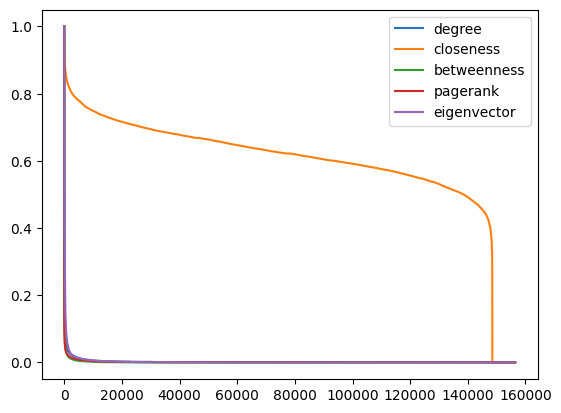
\includegraphics[width=.8\linewidth]{centrality_dists.png}
    \caption{Distribution of the centrality measures on the whole dataset. All values have been sorted in descending order and normalized.}
    \label{fig:centralities}
  \end{minipage}%
  \hspace{0.5cm}%
  \begin{minipage}{.48\textwidth}
    \centering
    %\captionsetup{justification=centering}
    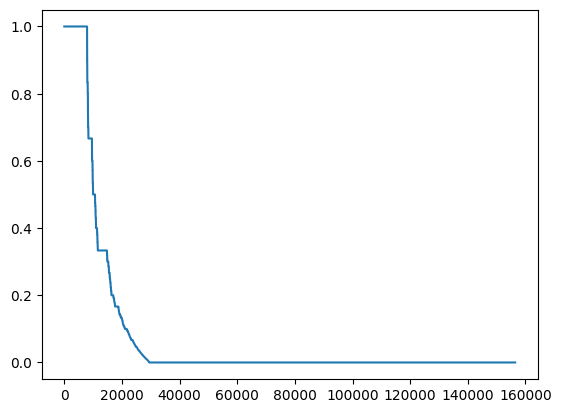
\includegraphics[width=.8\linewidth]{ccs_dists.png}
    \caption{Distribution of the local clustering coefficients on the whole dataset. All values have been sorted in descending order.}
    \label{fig:ccs}
  \end{minipage}
\end{figure*}

\begin{figure*}[]
  \centering
  \begin{subfigure}{.45\textwidth}
    \centering
    \captionsetup{justification=centering}
    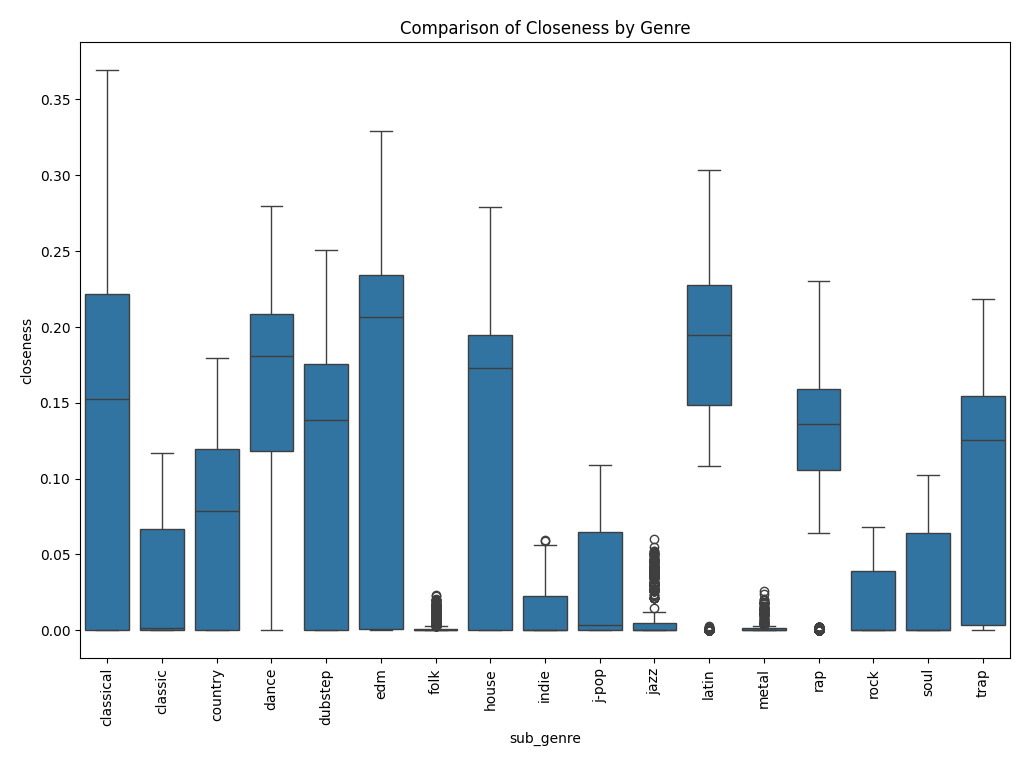
\includegraphics[width=\linewidth]{boxplot_closeness.png}  % Usa \includegraphics per il PDF
    \caption{Closeness centrality}
  \end{subfigure}
  \begin{subfigure}{.45\textwidth}
    \centering
    \captionsetup{justification=centering}
    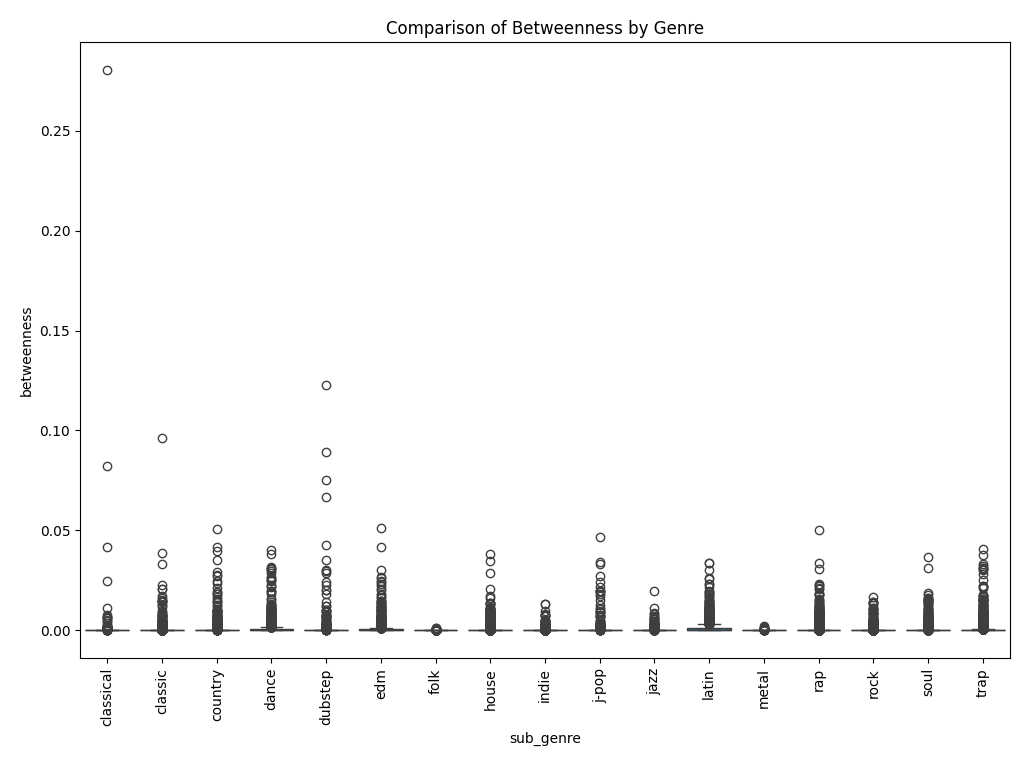
\includegraphics[width=\linewidth]{boxplot_betweenness.png}  % Usa \includegraphics per il PDF
    \caption{Betweenness centrality}
    \label{fig:between}
  \end{subfigure}
  \caption{Boxplots of the distribution of some centrality measures on several genre subgraphs.}
  \label{fig:boxplot}
\end{figure*}

\begin{figure*}[]
    \centering
    \captionsetup{justification=centering}
    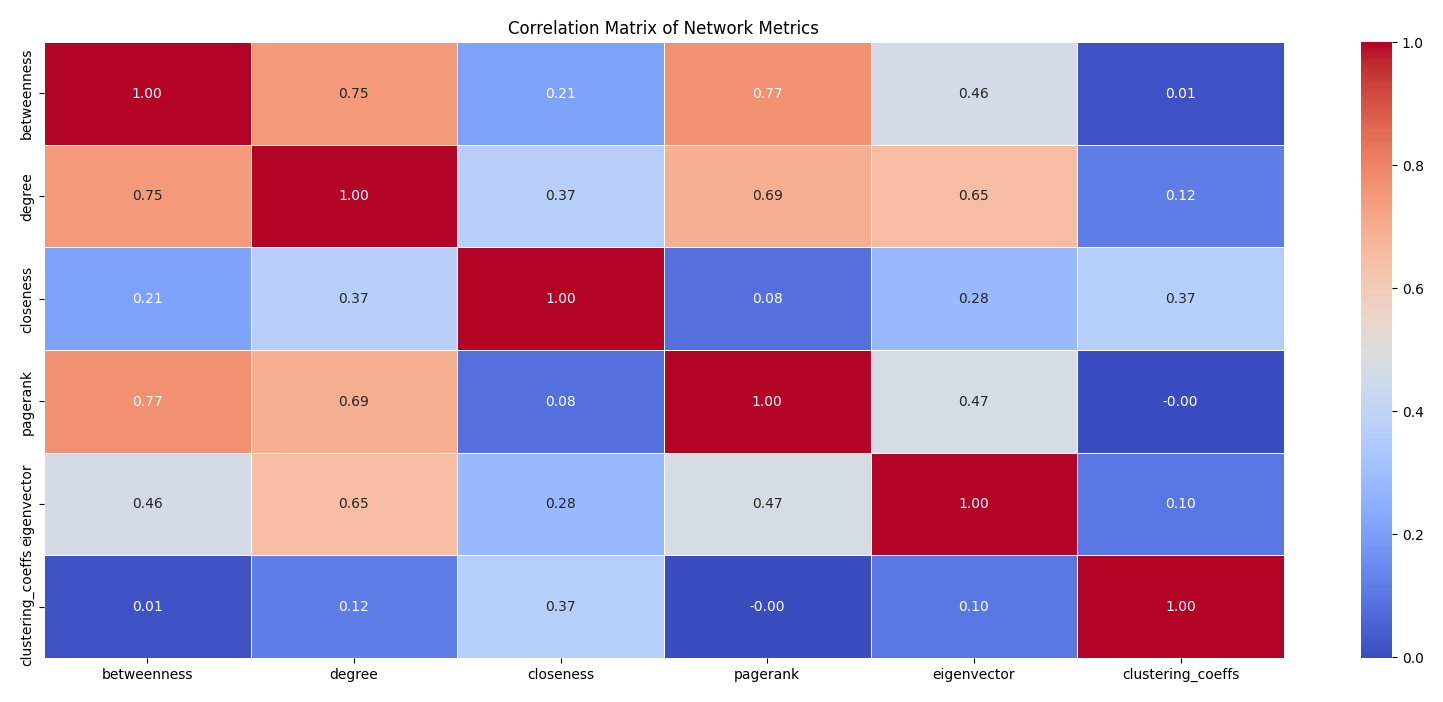
\includegraphics[width=.75\linewidth]{correlation.png}  % Usa \includegraphics per il PDF
    \caption{Correlation matrix between all node-level metrics computed on all genre subgraphs.}
    \label{fig:correlation}
\end{figure*}

\begin{figure*}[]
    \centering
    \begin{subfigure}{.33\textwidth}
      \centering
      \captionsetup{justification=centering}
      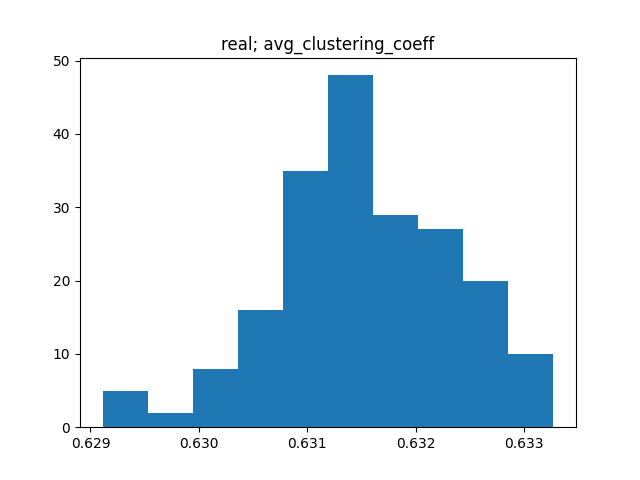
\includegraphics[width=\linewidth]{dist_plot_real_avg_clustering_coeff.png}
      \caption{Whole dataset, average \\ clustering coefficient}
      \label{fig:hist1}
    \end{subfigure}%
    \begin{subfigure}{.33\textwidth}
      \centering
      \captionsetup{justification=centering}
      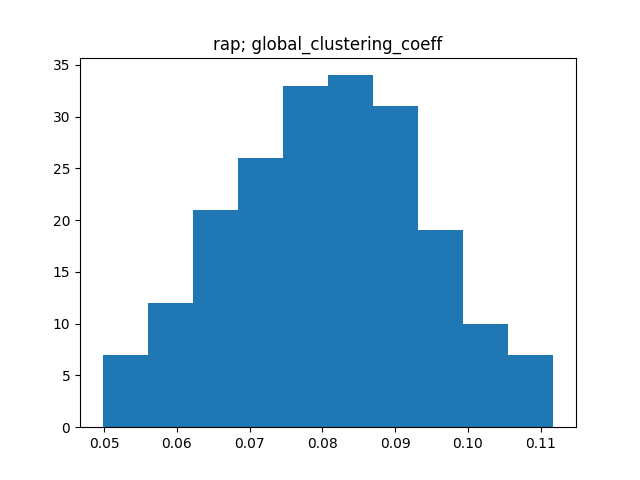
\includegraphics[width=\linewidth]{dist_plot_rap_global_clustering_coeff.png}
      \caption{Rap subgraph, global \\ clustering coefficient}
      \label{fig:hist2}
    \end{subfigure}
    \begin{subfigure}{.33\textwidth}
      \centering
      \captionsetup{justification=centering}
      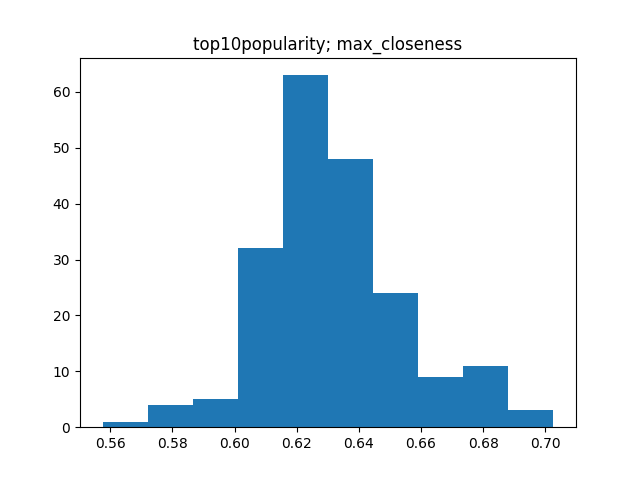
\includegraphics[width=\linewidth]{dist_plot_top10popularity_max_closeness.png}
      \caption{Top 10\% popularity subgraph, maximum closeness}
      \label{fig:hist3}
    \end{subfigure}
    \caption{Example of histograms for the metrics computed on random graphs that do not have a Gaussian distribution according to the Shapiro-Wilk test.}
    \label{fig:hist}
\end{figure*}